\begin{example}
    e.g. N-Queens in SAT. \vspace{7pt}

    Can we place in a $8 \times 8$ board $8$ queens without they attack each other? \vspace{3.5pt} 
    \begin{center}
        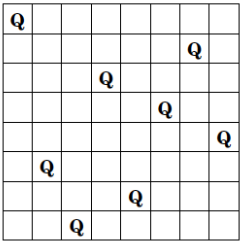
\includegraphics[width = 0.2\textwidth]{img/img29.png}
    \end{center} \vspace{3.5pt}

    \textbf{Boolean decision variables}. \\
    A boolean decision variable $p_{ij}$ describes each possible position on the board.
    \begin{itemize}
        \renewcommand{\labelitemi}{-}
        \item $p_{ij} = T$ means there is a queen on row $i$ and column $j$.
    \end{itemize} \vspace{7pt}

    \textbf{Constraints}.
    \begin{itemize}
        \renewcommand{\labelitemi}{-}
        \item Exactly one queen on each row. \vspace{3.5pt} \\
        The same condition can be expressed as the combination of two different constraints, which are:
        \begin{itemize}
            \item \textbf{At least one} queen on a row $i$. 
            $$ \forall i \in N, p_{i1} \vee \dots \vee p_{in} $$
            More synthetically: 
            $$ \forall i \in N, \bigvee_{1 \leq j \leq n} p_{ij} $$
            \item \textbf{At most one} queen on a row $i$.
            $$ \forall i \in N, \forall 0 < j < k \leq n, \neg (p_{ij} \wedge p_{ik}) $$
            Or more synthetically:
            $$ \forall i \in N, \bigwedge_{0 < j < k \leq n} \neg (p_{ij} \wedge p_{ik})$$
        \end{itemize}
        By \textbf{at least one} constraint we avoid that no queen is placed in a row, while by \textbf{at most one} constraint we force the solver to put only 
        one queen for each row.
        \item Exactly one queen on each column. \vspace{3.5pt} \\ 
        Column constraints are the same as the row constraints with $i$ and $j$ swapped.
    \end{itemize} \vspace{7pt}

    Therefore, we can combine together row and column constraints satisfying the generic form of the problem.
    \begin{itemize}
        \renewcommand{\labelitemi}{-}
        \item \textbf{At least one} queen on each row and column.
        $$ \bigwedge_{1 \leq i \leq n} \bigvee_{1 \leq j \leq n} p_{ij} $$
        $$ \bigwedge_{1 \leq j \leq n} \bigvee_{1 \leq i \leq n} p_{ij} $$
        \item \textbf{At most one} queen on each row and column.
        $$ \bigwedge_{1 \leq i \leq n} \bigwedge_{0 < j < k \leq n} \neg (p_{ij} \wedge p_{ik}) $$
        $$ \bigwedge_{1 \leq j \leq n} \bigwedge_{0 < i < k \leq n} \neg (p_{ij} \wedge p_{ik}) $$
    \end{itemize} \vspace{7pt}

    The reasoning about the diagonal constraints is a little bit different than before. \textbf{At most one} constraint is necessary, since two queens cannot 
    stay in the same diagonal. However, can we say the same thing for \textbf{at least one} constraint? We do not need at least one reasoning, since given a 
    diagonal there might not be a queen. \vspace{7pt}

    Additionally, we can detect if two or more queens share the same diagonal when the sum or the difference between their row and column indeces are the same.
    \begin{itemize}
        \renewcommand{\labelitemi}{-}
        \item $p_{ij}$ and $p_{i'j'}$ are on the same diagonal if and only if:
        $$ i + j = i' + j' \vee i - j = i' - j' $$
        \item \textbf{At most one} queen on each diagonal. 
        $$ \bigwedge_{1 \leq i < i' \leq n} \bigwedge_{j, j': i + j = i' + j' \vee i - j = i' - j'} \neg (p_{ij} \vee p_{i'j'}) $$
        This last constraint will take in account only those indeces such that the sums or the differences are the same, meaning the same diagonal.
    \end{itemize}
\end{example}
Generally, the SAT solver stops after the first solution given, so we lose the possibility to look at all the possible solutions. \vspace{7pt}

\textbf{How to find all solutions}? \\ 
After finding a solution, add the negation of it to the formula, and repeat this until the formula is UNSAT.